\documentclass[a4paper,12pt]{scrartcl}

\usepackage{bm,amsmath,url,graphicx}
\usepackage{palatino}
\usepackage{color, xcolor}
\usepackage{listings}


\newcommand{\n}{\mathbf{ n}}
\newcommand{\h}{\mathbf{ h}}
\newcommand{\x}{\mathbf{ x}}
\newcommand{\y}{\mathbf{ y}}
\newcommand{\w}{\mathbf{ w}}
\newcommand{\HH}{\mathbf{ H}}
\newcommand{\R}{\mathbf{ R}}
\newcommand{\C}{\mathbf{ C}}
\newcommand{\thb}{{\boldsymbol{\theta}}}
\newcommand{\mub}{{\boldsymbol{\mu}}}
\newcommand{\python}{{\fbox{\texttt{\bfseries python}}\quad}}
\newcommand{\pen}{{\fbox{\texttt{\bfseries pen\&paper}}\quad}}

\renewcommand{\familydefault}{\rmdefault}


\begin{document}
\section*{SGN-41007 Pattern Recognition and Machine Learning}
\emph{Exercise Set 5: February 8--February 10, 2017}
\bigskip
\sloppy

\lstdefinestyle{mystyle}{
  belowcaptionskip=1\baselineskip,
  breaklines=true,
  frame=single,
  xleftmargin=\parindent,
  language=Python,
  showstringspaces=false,
  basicstyle=\ttfamily,
  keywordstyle=\bfseries\color{green!40!black},
  commentstyle=\itshape\color{purple!40!black},
  identifierstyle=\color{blue},
  stringstyle=\color{orange},
  moredelim=**[is][\color{red}]{@}{@},
}

\lstset{language=Python,style=mystyle} 


\noindent
Exercises consist of both pen\&paper and computer assignments.
Pen\&paper questions are solved at home before exercises, while
computer assignments are solved during exercise hours. The
computer assignments are marked by  \python and 
Pen\&paper questions by  \pen

\begin{enumerate}

\item \pen \emph{Derive the explicit mapping corresponding to a kernel trick.}

In the lectures we saw that the kernel trick $\kappa(\x, \y) = (\x \cdot \y)^2$
for $\x = (x_1,x_2)$ and $\y = (y_1,y_2)$ corresponds to the mapping 
\[
\begin{pmatrix}
u \\ v
\end{pmatrix}
\mapsto 
\begin{pmatrix}
u^2\\
v^2\\
\sqrt{2}u v
\end{pmatrix}
\]
Find the explicit mapping corresponding to the inhomogeneous kernel
$\kappa(\x, \y) = (\x \cdot \y + 1)^2$ with $\x, \y\in\R^2$.

\emph{Hint:} Expand the kernel formula as far as you can. 
At that point, reformulate the result into a dot product of
two 5-dimensional vectors; one composed of coordinates of $\x$ only
and the other of coordinates of $\y$ only.

\item \pen \emph{Compute the gradient of the log-loss.}

In the lectures we defined the \emph{logistic loss function}:
\begin{equation}
\ell(\w) = \sum_{n = 0}^{N-1} \ln(1 + \exp(-y_n\w^T\x_n)).
\label{eq:grad}
\end{equation}
Note that there was a typo in the slides with minus sign missing from the $\exp()$ function.

\begin{enumerate}
	\item Compute the formula for its gradient $\frac{\partial \ell(\w) }{\partial \w}$.
	\item There are two alternative strategies for using the gradient.
	\begin{itemize}
		\item \textbf{Batch gradient:} Compute the gradient from all samples and then apply the gradient descent rule
		$\w \leftarrow \w - \eta \frac{\partial \ell(\w) }{\partial \w}$.
		\item \textbf{Stochastic gradient:} Compute the gradient from one sample and then apply the gradient descent rule.
		In other words, pretend $N = 1$ in formula \ref{eq:grad}.
	\end{itemize}
	In the latter case, compute the next estimate for $\w$ when $\x_n = [-0.3, -1.7]^T$ and
	$y[n] = 1$ and $\w =[  0.9,  0.9]^T$.
\end{enumerate}

\item \python \emph{Implement gradient descent for log-loss.}

\begin{enumerate}
\item Implement a log-loss minimization algorithm. You may use the template provided by the
teaching assistant.
\item Apply the code for the data downloaded from

\url{https://github.com/mahehu/SGN-41007/tree/master/exercises/Ex5/log_loss_data.mat}

The data is in Matlab format. Load it as follows:
\begin{verbatim}
from scipy.io import loadmat
data = loadmat("log_loss_data.mat")
\end{verbatim}

After this, \verb+data+ is a dict object (similar to \verb+map+ in C++).
You can see the contents by:
\begin{verbatim}
>>> data.keys()
['y', 'X']
\end{verbatim}
and access the contents as:
\begin{verbatim}
>>> X = data["X"]
>>> print X.shape
(400L, 2L)
\end{verbatim}

\item Plot the path of $\w$ over 100 iterations and check the accuracy (see plots below).

\end{enumerate}

\centerline{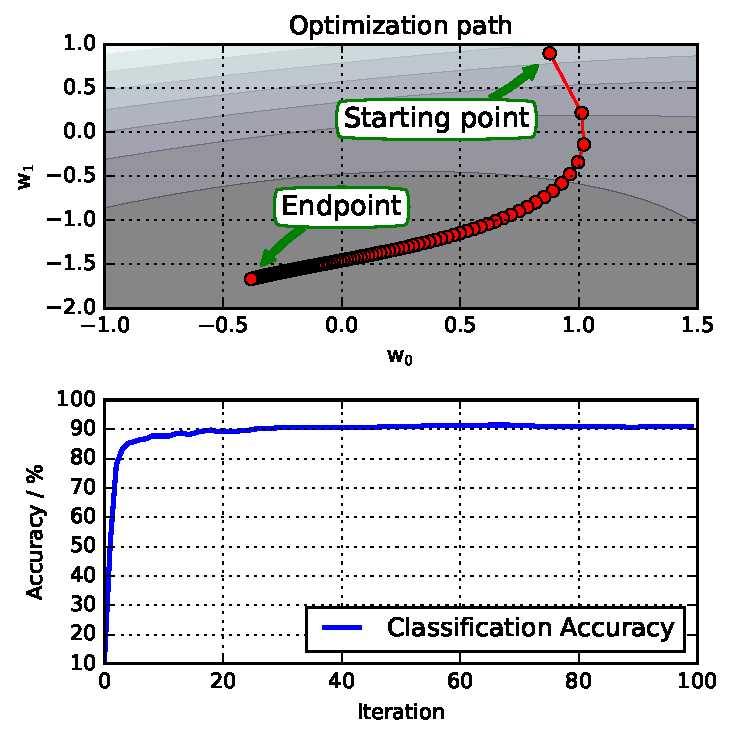
\includegraphics[width=0.5\textwidth]{log_loss_minimization.pdf}}

\item \python \emph{Select appropriate hyperparameters for the GTSRB data.}

Last week we trained classifiers for the German Traffic Sign
Recognition Benchmark (GTSRB) dataset. It turned out that the SVM was
really poor with default arguments, but changing the kernel pushed it
to the top. In this exercise, we use brute force to find good hyperparameters
for the classifiers (kernel, C, number of trees, etc.).

Consider the following two classifiers
	\begin{verbatim}
clf_list = [LogisticRegression(), SVC()]
clf_name = ['LR', 'SVC']
	\end{verbatim}
	Most important hyperparameters are the \emph{regularization strength} \verb+C+ and
	the penalty type parameter \verb+penalty+, which can have values "\verb+l1+" and "\verb+l2+".
	
	In order to use the same range for the two methods, you need to scale the data to
	zero mean and unit variance using \verb+sklearn.preprocessing.Normalizer+.
	
	Implement
	a grid search over these two parameters along the following lines:
	\begin{verbatim}
for clf,name in zip(clf_list, clf_name):
    for C in C_range:
		    for penalty in ["l1", "l2"]:
            clf.C = C
            clf.penalty = penalty
            clf.fit(X_train, y_train)
            y_pred = clf.predict(X_test)
            score = accuracy_score(y_test, y_pred)
\end{verbatim}
A reasonable range for \verb+C+ is $C\in\{10^{-5},...,10^{0}\}$.

\item \python \emph{Train ensemble methods with the GTSRB data.}

\begin{enumerate}
\item Train a 100-tree Random Forest classifier with the GTSRB and compute the accuracy on the test set.
\item Train a 100-tree Extremely Randomized Trees classifier with the GTSRB and compute the accuracy on the test set.
\item Train a 100-tree AdaBoost classifier with the GTSRB and compute the accuracy on the test set.
\item Train a 100-tree Gradient Boosted Tree classifier with the GTSRB and compute the accuracy on the test set.
\end{enumerate}


\end{enumerate}

\end{document}          
